\Chapter{Klaszterezés}

Ahhoz, hogy szürkeárnyalatos képeket megfelelően tudjunk kiszínezni, első lépésként meg kell határoznunk a kiszínezendő területeket. El kell döntenünk hogy a kép mely részei tartoznak ugyan ahhoz a színárnyalathoz és melyek nem. Ezek alapján a dolgozat 2 fő részre bontható:
\begin{itemize}
\item képszegmentálás
\item szegmensek kiszínezése
\end{itemize}

A képszegmentálás célja az, hogy a képen lévő különböző célterületeket elkülönítse, a klaszterezés célja pedig az azonos tulajdonságokkal rendelkező objektumok közös kategóriába sorolása ahol az egy kategóriába tartozó objektumok egymáshoz hasonlóak, viszont különböznek a többi kategóriában lévő objektumoktól.

A két módszer célja lényegében megegyezik egymással. Ahhoz hogy a képből ki tudjuk nyerni a megfelelő szegmenseket, valamilyen klaszterezési eljárást kell alkalmaznunk.

A klaszterezési algoritmusokat a következő módon tudjuk csoportosítani\cite{clustering}:
\begin{itemize}
\item hierarchikus: a korábban létrehozott klaszterek felhasználásával találja meg az egymást követő klasztereket
    \begin{itemize}
    \item agglomeratív (bottom-up): minden egyes elemet különálló klaszterként kezel és azokat nagyobb klaszterekbe egyesíti
    \item osztó (top-down): a teljes halmazból indul ki és azt kisebb klaszterekre osztja
    \end{itemize}
\item particionáló: egyszerre határozza meg az összes klasztert
\item rács alapú: a teret véges számú cellára kvantálja amelyek egy rácsszerkezetet alkotnak, és ezeken hajtja végre a klaszterezést
\item modell alapú: megpróbálja az adatokat optimálisan ráilleszteni valamilyen matematikai modellre
\end{itemize}

A kutatások során az egyik legnépszerűbb particionáló klaszterezést használtam, a k-means klaszterezést.

\Section{K-means klaszterezés}

\begin{python}
def kmeans_segmentation(image, k):
    """
    Segmenting the image using opencv-python's k-means method
    :param image: the image that I want to carry out the segmentation
    :param k: the number of the clusters
    :return: the compactness, the pixel_values and the labels
        from the k-means method
    """
    pixel_values = image.reshape((-1, 1))
    pixel_values = np.float32(pixel_values)

    criteria = \
        (cv2.TERM_CRITERIA_EPS + cv2.TERM_CRITERIA_MAX_ITER, 100, 0.2)

    compactness, labels, (centers) = cv2.kmeans(
        pixel_values,
        k,
        None,
        criteria,
        10,
        cv2.KMEANS_RANDOM_CENTERS)

    labels = labels.flatten()

    return compactness, pixel_values, labels
\end{python}

\Section{Optimális klaszterszám meghatározása}

Az optimális klaszterszám meghatározásához 4 módszert teszteltem le, ezeknek az eredménye a következő alfejezetekben található.
A módszereket a \cite{tomatoleaf} és a \cite{elbow} kutatások alapján választottam.

\SubSection{Silhouette módszer}

A Silhouette index azt méri, hogy egy adott objektum mennyire hasonlít a saját klaszterében lévő objektumokhoz. Az értéke +1 és -1 között mozog. A nagyobb érték azt jelzi hogy az objektum jól illeszkedik a saját klaszteréhez és rosszul illeszkedik a szomszédos klaszterekhez. Ha a legtöbb obbjektumnak pozitív az értéke akkor a klaszterezés megfelelő, ha sok objektumnak negatív, akkor vagy túl sok a klaszter, vagy túl kevés. A módszer a következő képlettel írható le:

\[ S(k)=\frac{1}{num} \sum_{i=1}^{num} \frac{b(i)-a(i)}{max\{a(i),b(i)\}} \quad \cite{tomatoleaf} \]

ahol
\begin{itemize}
\item $n$: a klaszterek száma
\item $num$: a pixelek száma
\item $a(i)$: az $i$ minta és az ugyanabban a klaszterben lévő többi minta közötti átlagos távolság
\item $b(i)$: az $i$ minta és az összes többi klaszter mintája közötti távolság minimális értéke
\end{itemize}
Ennek eredményeként megkapjuk a Silhouette pontszámot. Ha elvégezzük ezt a vizsgálatot különböző klaszterszámokra, akkor amelyiknek a pontszáma a legnagyobb, az lesz a legoptimálisabb klaszterszám. 

Vizsgálataim során a \texttt{sklearn.metrics} csomagban található \texttt{silhouette\_score} módszert használtam a következő kódrészletben látható módon. Ez a metódus megtalálható az általam készített \texttt{commonmethods} csomagban.
\begin{python}
def silhouette_method(values, labels):
    """
    Calculating the Silhouette method for the given values with
    the given labels, and measuring time.
    :param values: in my case the pixel values from the k-means method
    :param labels: in my case the labels from the k-means method
    :return: the time of the calculation and
        the calculated Silhouette score
    """
    start = time.time()
    s_score = silhouette_score(values, labels)
    end = time.time()

    s_time = end-start

    return s_time, s_score
\end{python}
Mint látható, a metódus visszatér a módszer számítási idejével, mivel a vizsgálataim során a futási idők összevetése volt az egyik fő szempont. Ezen kívül visszaadja a kiszámított Silhouette pontszámot is, amit az általam megadott értékekből és a hozzájuk tartozó címkékből állít elő. Ezeket az értékeket a \texttt{kmeans\_segmentation} metódus eredményeként kapom.

A Silhouette módszer esetén azt tapasztaltam, hogy a futási ideje elég lassú. A \ref{fig:silhouette_runtime} ábrán látható a módszer futási ideje különböző méretű képekre.

\begin{figure}[h]
\centering
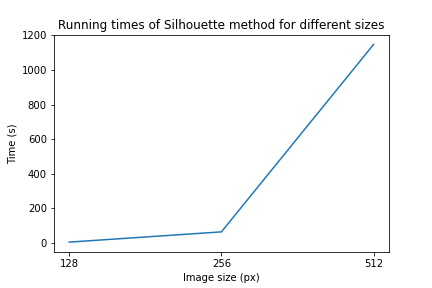
\includegraphics[scale=0.9]{images/silhouette_runtime.png}
\caption{A Silhouette módszer futási ideje különböző képméretekre.}
\label{fig:silhouette_runtime}
\end{figure}

\SubSection{Davies-Bouldin módszer}
A Davies-Bouldin index a klaszteren belüli szóródás összegének és a klaszterek közötti szétválás arányának a függvénye. A célunk az, hogy ezt az értéket minimalizáljuk, hiszen azt szeretnénk hogy a klaszteren belüli szórás minimális, a klaszterek közötti elkülönülés pedig maximális legyen.

A módszer képlete a következő:

\[ DB(k)=\frac{1}{k} \sum_{i=1}^{K} max \left(\frac{W_i + W_j}{C_{ij}}\right)  \quad \cite{tomatoleaf} \]

ahol
\begin{itemize}
\item $K$: a klaszterek száma
\item $W_i$: a $C_i$ osztályba tartozó összes minta átlagos távolsága a klaszter középpontjától
\item $W_{j}$: a $C_i$ osztályba tartozó összes minta átlagos távolsága a $C_j$ osztály középpontjától 
\item $C_{ij}$: a $C_i$ és $C_j$ osztályok középpontja közötti távolság
\end{itemize}
Ennek eredményeként megkapjuk a Davies-Bouldin pontszámot. Ha elvégezzük ezt a vizsgálatot különböző klaszterszámokra, akkor amelyiknek a pontszáma a legkisebb, az lesz a legoptimálisabb klaszterszám.

Ennek a módszernek a megvalósításához a \texttt{sklearn.metrics} csomagban található \texttt{davies\_bouldin\_score} metódust használtam. A következő kódrészletben látható hogy, a módszer megvalósítása ugyan arra a sémára épül, mint a \texttt{silhouette\_method}. Ez a metódus is megtalálható az általam készített \texttt{commonmethods} csomagban.
\begin{python}
def davies_bouldin_method(values, labels):
    """
    Calculating the Davies-Bouldin method for the given values with
    the given labels, and measuring time.
    :param values: in my case the pixel values from the k-means method
    :param labels: in my case the labels from the k-means method
    :return: the time of the calculation and
        the calculated Davies-Bouldin score
    """
    start = time.time()
    db_score = davies_bouldin_score(values, labels)
    end = time.time()

    db_time = end-start

    return db_time, db_score
\end{python}

\SubSection{Calinski-Harabasz módszer}

A Calinski-Harabasz indexet belső klaszterérvényességi mérőszámként szokták használni, amely a létrehozott klasztereket osztályozza.

A módszer képlete a következő \cite{silhouette_calinski}:

\begin{equation*}
\begin{split} \label{}
 CH(k) & =\frac{B(K)(N-K)}{W(K)(K-1)} \\
 & B(K)=\sum_{k=1}^{K}a_k \|\overline{x_k}-\overline{x}\|^2 \\
 & W(K)=\sum_{k=1}^{K}\sum_{C(j)=k}\|x_j-\overline{x_k}\|^2
\end{split}
\end{equation*}

ahol
\begin{itemize}
\item $K$: a klaszterek száma
\item $N$: a minta száma
\item $B(K)$: a klaszterek közötti divergencia, más néven a klaszterek közötti kovariancia
\item $W(K)$: a klaszteren belüli divergencia, más néven a klaszteren belüli kovariancia
\end{itemize}

Minél nagyobb a $B(K)$ értéke, annál nagyobb a klaszterek közötti diszperzió mértéke. Minél kisebb a $W(K)$ értéke, annál szorosabb a kapcsolat a klaszteren belül. Minél nagyobb az arány, annál nagyobb a Calinski-Harabasz pontszám értéke, theát annál optimálisabb a klaszterszám.

Ennek a módszernek a megvalósításához a \texttt{sklearn.metrics} csomagban található \texttt{calinski\_harabasz\_score} metódust használtam. A következő kódrészletben látható hogy, a módszer megvalósítása ugyan arra a sémára épül, mint a \texttt{silhouette\_method} és a \texttt{davies\_bouldin\_method}. Ez a metódus is megtalálható az általam készített \texttt{commonmethods} csomagban.
\begin{python}
def calinski_harabasz_method(values, labels):
    """
    Calculating the Calinski-Harabasz method for the given values with
    the given labels, and measuring time.
    :param values: in my case the pixel values from the k-means method
    :param labels: in my case the labels from the k-means method
    :return: the time of the calculation and
        the calculated Calinski-Harabasz score
    """
    start = time.time()
    ch_score = calinski_harabasz_score(values, labels)
    end = time.time()

    ch_time = end-start
\end{python}

\SubSection{Elbow módszer}

Módszer, futási nehézségek.

\SubSection{Összegzés}

A méretek szerinti futási eredményeket a \aref{tab:size_runtimes}. táblázat tartalmazza.

\begin{table}[h]
\centering
\caption{Futási idők átlaga különböző módszerek esetén}
\label{tab:size_runtimes}
\medskip
\begin{tabular}{|l|c|c|c|c|}
\cline{2-5}
 \multicolumn{1}{c|}{} & \multicolumn{4}{c|}{Kép mérete} \\
 \hline
 Módszer & 64px & 128px & 256px & 512px \\
\hline
Silhouette módszer & 0.2684s & 4.4029s & 68.0697s & 1183.2937s \\
Davies-Bouldin módszer & 0.0071s & 0.0042s & 0.0096s & 0.0274s \\
Calinski-Harabasz módszer & 0.0031s & 0.001s & 0.0028s & 0.0120s \\
\hline
\end{tabular}
\end{table}

A klaszterszám szerinti futási eredményeket a \aref{tab:cluster_runtimes}. táblázat tartalmazza.

\begin{table}[h]
\centering
\caption{Futási idők átlaga különböző klaszterszámok és módszerek esetén, 256px képméretre}
\label{tab:cluster_runtimes}
\medskip
\begin{tabular}{|l|c|c|c|}
\cline{2-4}
 \multicolumn{1}{c|}{} & \multicolumn{3}{c|}{Klaszterek száma} \\
 \hline
 Módszer & 2 & 4 & 8 \\
\hline
Silhouette módszer & 63.1462s & 63.1254s & 62.2278s \\
Davies-Bouldin módszer & 0.0060s & 0.0083s & 0.0064s \\
Calinski-Harabasz módszer & 0.0026s & 0.0024s & 0.0028s \\
\hline
\end{tabular}
\end{table}
